\mychapter{1}{Introducción}

El objetivo de este proyecto es la predicción temprana de la enfermedad de Alzheimer a partir de imágenes biomédicas de pacientes en distintos estados de la endermedad. Este proceso de predicción se realizará utilizando técnicas que se engloban dentro del Deep Learning.

\section{Motivación}

Actualmente, la enfermadad de Alzheimer es la principal causa de demencia en el ser humano. Lo que se produce es un deterioro progresivo de las celulas nerviosas cerebrales, lo que desemboca en demencia senil. El aumento de Apersonas afectadas por esta enfermedad viene dado en parte por el aumento de la esperanza de vida, ya que esta enfermedad se da en personas de edad avanzada. Las consecuencias de esta enfermedad son varias, pero todas limitan la calidad de vida de la persona que la padece, además del de las personas de su entorno, ya que esta enfermedad va minando la autonomía del enfermo sobre su propio cuerpo. Esto provocará que el enfermo necesite un apoyo externo para poder realizar su día a día.\\

Aún no se sabe la causa de la enfermedad de Alzheimer, aunque si se conocen factores de riesgo que pueden ayudar a su desarrollo \cite{RiskFactors}. Los principales que se conocen son los siguientes: la edad (como se ha explicado antes con el aumento de la esperanza de vida), el sexo (afectando más a mujeres que a hombres), el nivel de eduación (las personas con estudios y mayor actividad intelectual son menos propensas a esta enfermedad), los trastornos metabólicos asociados con la resistencia a la insulina, la obesidad, hipertensión o diabetes y la genética (la presencia del genotipo determinado del gen de la EPOE) entre otros factores.\\
No existe una cura de la enfermedad, solo se conocen tratamientos que relentizan su avance. Estos tratamientos deben realizarse en las primeras fases de la enfermedad, ya que después pueden resultar perjudiciales para el paciente.\\

El diagnóstico del Alzheimer se podría dividir en tres partes \cite{Diagnostico}:
\begin{itemize}
	\item \textbf{Evaluación de estado de ánimo y estado mental:} El estado mental se evalúa para darle al médico una idea general de qué tan bien está funcionando la mente. Este examen da un sentido general sobre si la persona: está consciente de que tiene síntomas. sabe la fecha, la hora, y dónde está ella, puede recordar una lista corta de palabras, seguir instrucciones y hacer cálculos simples. El doctor puede que le pregunte a la persona su dirección, qué año es y quién es el presidente del país. Puede que al individuo se le pida que deletree una palabra al revés, que dibuje un reloj y que copie un diseño. El doctor también puede evaluar el estado de ánimo y el sentimiento de bienestar de la persona para detectar si hay depresión u otra enfermedad que puede causar pérdida de memoria y confusión.
	\item \textbf{Examen físico y exámenes para el diagnóstico}: El doctor hará ciertos procedimientos para evaluar la salud en general de la persona como su dieta, tomar la presión arterial, o escuchar su corazón. Se harán pruebas de sangre y de orina y posiblemente se ordenen otros exámenes de laboratorio. La información que pueden proporcionar estos exámenes puede ayudar a identificar problemas como anemia, diabetes, problemas de los riñones o del hígado, deficiencias de vitaminas, anormalidades de la tiroides y problemas del corazón o de los vasos sanguíneos. Todas estas condiciones pueden causar confusión, problemas de memoria u otros síntomas similares a la Demencia.
	\item \textbf{Examen neurológico:} Un doctor o a veces un Neurólogo que se especializa en problemas del cerebro y del sistema nervioso, evaluará muy cuidadosamente a la persona para determinar si hay señales de otro tipo de problema del cerebro que no es Alzheimer. El doctor también va a evaluar los reflejos de la persona, el equilibrio, movimiento de los ojos, lenguaje y sensibilidad. El doctor está buscando señales de derrames pequeños o grandes, enfermedad de Parkinson, tumores cerebrales, acumulación de líquido en el cerebro y otros males que pueden perjudicar la memoria o la capacidad de pensar. El examen neurológico puede incluir un MRI (Imagen por Resonancia Magnética) o CT (tomografía computarizada). Los MRI y CT pueden revelar tumores, evidencia de derrames pequeños o grandes, daño a causa de lesiones por traumas severos de cabeza o acumulación de líquido. Medicare cubre el PET (tomografía por emisión de positrones) como una ayuda para el diagnóstico en ciertos casos .
\end{itemize}

El análisis de la imagen de resonancia magnética a través del ojo humano resulta sencillo si las alteraciones estructurales son apreciables. Normalmente se utiliza una escala de grises para poder resaltar las diferencias \cite{FormatosImagenes}. El número de bits con el que trabajan estos sistemas suele ser de 16 bits \cite{FormatosImagenes} lo cuál da una escala de grises de hasta 65536 niveles, muy superior a los niveles que el ojo puede diferenciar.\\

Para tener un estudio más exhaustivo del estado del paciente, se aplican una serie de algoritmos de ordenador para poder extraer las zonas de mayor interés que son las que observa el evaluador para poder determinar si existen indicios de la enfermedad en el paciente. El principal problema es que si nos encontramos en el inicio de la enfermedad, pueden no existir una alteración suficiente para poder diagnosticar la enfermedad por el ojo humano. He aquí la motivación de la realización del proyecto, poder ayudar a un diagnóstico temprano de la enfermadad para poder tratarla con procedimientos que reduzcan su avance, y mejoren la vida del paciente.

\section{Alzheimer}

La \textbf{enfermedad de Alzheimer (EA)}  es una enfermedad neurodegenerativa que se manifiesta como deterioro cognitivo y trastornos conductuales. Se caracteriza, en la mayoría de ocasiones,  por una perdida de memoria inmediata  y de otras capacidades mentales, a medida que mueren las células nerviosas(neuronas) y se atrofian diferentes zonas del cerebro. La enfermedad suele tener una duración media de aproximada después del diagnóstico al paciente de unos 10 años, todo dependiendo por supuesto de la etapa en la que se diagnostique la enfermedad.\\

La enfermedad de Alzheimer es la forma más común de demencia, es incurable y terminal, y aparece con mayor frecuencia en personas mayores de 65 años de edad \cite{3}, aunque en otros casos más raros y extremos puede ser desarrollada a partir de los 40 años. \\

Los síntomas de la enfermedad como una enfermedad nosológica fueron definidos por primera vez por \textbf{Emil Kraepelin} (Neustrelitz, 15 de febrero de 1856 – Múnich, 7 de octubre de 1926), mientras que la neuropatología característica fue observada por primera vez por \textbf{Alois Alzheimer} (Marktbreit, 14 de junio de 1864 - Breslavia, 19 de diciembre de 1915) en 1906. Ambos trabajaban en el mismo laboratorio, por lo que se puede considerar que el descubrimiento fue obra de ambos psiquiatras. Pero dado a que Kraepelin daba mucha importancia a encontrar la base neuropatológica de los desordenes psiquiátricos, decidió nombrar la enfermedad Alzheimer en honor a su compañero.\\


Normalmente, el síntoma inicial es una perdida de la habilidad para adquirir nuevos recuerdos, y esto suele confundirse con actitudes relacionadas con la vejez o el estrés, ya que es en esta etapa de la vida en la que se suele desarrollar la enfermedad.Ante la sospecha de alzhéimer, el diagnóstico se realiza con evaluaciones de conductas cognitivas, así como neuroimágenes, de estar estas disponibles.\\

A medida que la enfermedad va progresando, aparecen la confusión mental,irratibilidad y agresión, cambios de humor, transtornos del lenguaje, pérdida de la memoria a corto plazo y una predisposición a aislarse a medida que declinan los sentidos del paciente. Finalmente se pierden funciones biológicas, lo que conlleva la muerte.\\

La causa de la enfermedad permanece desconocida \label{desconocida}, aunque las últimas investigaciones parece indicar que se encuentran implicados procesos de tipo priórico\cite{4}.  Las investigaciones suelen asociar la enfermedad a la aparición de placas seniles y ovillos neurofibrilares. Hoy en día, los tratamientos que se ofrecen moderados beneficios sintomáticos, pero no hay tratamiento que retrase o detenga el progreso de la enfermedad.\\

Según el siguiente estudio  \cite{populationofalzheimerinSpain}, en España podemos encontrar la siguiente tabla con respecto a la población que padece esta enfermedad:
\begin{table}[h]
	\centering
	\begin{tabular}{|l|l|}
		\hline
		Edad  & \begin{tabular}[c]{@{}l@{}}Indidencia\\ (nuevos casos)\\ por cada mil personas\end{tabular} \\ \hline
		65-69 & 3                                                                                           \\ \hline
		70-74 & 6                                                                                           \\ \hline
		75-79 & 9                                                                                           \\ \hline
		80-84 & 23                                                                                          \\ \hline
		85-89 & 40                                                                                          \\ \hline
		90-   & 69                                                                                          \\ \hline
	\end{tabular}
	\caption{Incidencias de la enfermedad en España respecto a la edad \cite{populationofalzheimerinSpain}}
	\label{tabla1}
\end{table}

\subsection{Definiciones}

Dentro de la enfermedad, se pueden distinguir 4 tipos de pacientes:\\

\begin{itemize}
	\item \textbf{AD: } Acrónimo para un paciente que padece la enfermedad de Alzheimer.
	\item \textbf{LMCI: } Acrónimo para \textit{" Late Mild cognitive impairment"}.  El \textbf{Mild Cognitive Impairment}  es una entidad nosológica que pretende describir la sintomatología previa al Alzheimer. En este caso, el Late inicial indica que se encuentra en una fase avanzada de este estado previo a poder diagnosticar que el paciente sufre Alzheimer.
	\item \textbf{EMCI: } Acrónimo para \textit{" Early Mild cognitive impairment"}.  En este caso, el Early inicial indica que se encuentra en una fase temprana de este estado previo a poder diagnosticar que el paciente sufre Alzheimer.
	\item \textbf{Normal: } Este termino se utiliza para hablar de un paciente el cuál no sufre la enfermedad.
\end{itemize}

Como se ha explicado previamente, cuanto antes se encuentren señales de un desarrollo de la enfermedad, antes se podrá actuar para el tratamiento de la misma lo cual conlleva una mejor situación de vida para el paciente.\\

Esto implica que el principal grupo de estudio, es el de los pacientes \textbf{MCI.}  Las causas del MCI puede ser agrupadas en enfermedades neurológicas, desordes en el sistema, factores tóxicos o de medicación, factores psiquiátricos o una combinación de los anteriores, como se pueden observar en 
\cite{pertersen2007}.

\begin{figure}[h]
	\label{figure1}
	\centering
	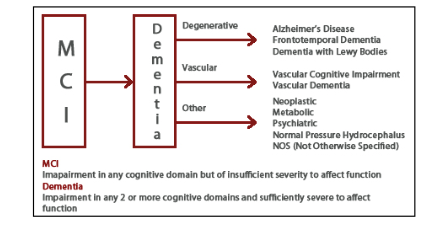
\includegraphics[width=\textwidth]{imagenes/figure1.png}
	\caption{Caracterización de MCI que precede al diagnóstico de la enfermedad de Alzheimer}
\end{figure}

Aún así, el grupo de pacientes más difícil de clasificar es este, ya que si se encuentra en la fase de \textbf{EMCI}, es difícil diferenciarlo de un paciente normal que presenta síntomas de perdida de tejido cerebral propio de la edad avanzada que de un paciente que está comenzando a padecer le enfermedad de Alzheimer.\\

\section{Resumen y estructura del proyecto}

Con este proyecto se intenta responder a 2 preguntas principales. La primera pregunta es si con estas técnicas podemos realizar una clasificación correcta de imágenes 2D cerebrales de pacientes y la segunda pregunta es que de ser así, cuáles serían las capas del cerebro más favorables a la hora de realizar esta clasificación.\\

Para responder a estas preguntas se deben llevar a cabo distintas fases como el procesamiento de las imágenes en 3D para obtener imágenes 2D cerebrales, la elección de una arquitectura de red neuronal, la elección de los distintos métodos de validación y la elección de los experimentos para poder responder a estas dos preguntas.\\

La estructura del proyecto es la siguiente:
\begin{enumerate}
	\item \textbf{Introducción: }En este caso se ha explicado brevemente la motivación a la hora de la realización de este proyecto además de un breve repaso de la enfermedad de Alzheimer.
	\item \textbf{Objetivos: }En este capítulo se hablará de los objetivos que se desean conseguir en la realización de este proyecto.
	\item \textbf{Fundamento del proceso implementado: }En este capítulo se explicará teóricamente la base de las herramientas que se han utilizado para la realización del proyecto y la obtención de sus resultados.
	\item \textbf{Análisis del diagnóstico de la enfermedad de Alzheimer: } En este articulo se realizará un repaso a la bibliografía existente sobre los factores más notables a la hora de predicción de la enfermedad tanto en el ámbito médico como con el uso de ordenadores. 
	\item \textbf{Análisis y Desarrollo Experimental: }En este capítulo se explicarán cuáles han sido las máquinas en las que se ha realizado el grueso del proyecto, cuáles han sido los elementos comunes a todos los experimentos y cuáles son los experimentos que se han realizado para responder a las preguntas que nos realizábamos al comienzo del mismo.
	\item \textbf{Base de Datos: }En este capítulo se hablará de la base de datos que ha sido utilizada y cómo está estructurada, además del post procesamiento que han recibido las imágenes de la base de datos que se ha utilizado.
	\item \textbf{Resultados: }En este capítulo se hablará de los resultados obtenidos en los distintos experimentos.
	\item \textbf{Conclusiones y Trabajos Futuros: }En este último capítulo se comentarán las conclusiones que se han podido obtener con los experimentos y posibles continuaciones que se desean realizar a partir de lo obtenido en este proyecto.
\end{enumerate}